\documentclass[english,11pt]{beamer}

\DeclareMathOperator{\Cov}{Cov}
\DeclareMathOperator{\Var}{Var}
\DeclareMathOperator{\E}{\mathbb{E}}
\DeclareMathOperator{\Proba}{\mathbb{P}}

\newcommand{\Covb}[2]{\ensuremath{\Cov\!\left[#1,#2\right]}}
\newcommand{\Eb}[1]{\ensuremath{\E\!\left[#1\right]}}
\newcommand{\Pb}[1]{\ensuremath{\Proba\!\left[#1\right]}}
\newcommand{\Varb}[1]{\ensuremath{\Var\!\left[#1\right]}}

% norm
\newcommand{\norm}[1]{\| #1 \|}

\newcommand{\indep}{\rotatebox[origin=c]{90}{$\models$}}





\usepackage{mathptmx,amsmath,amssymb,graphicx,bibentry,bbm,babel,ragged2e}

\makeatletter

\newcommand{\noun}[1]{\textsc{#1}}
\newcommand{\jitem}[1]{\item \begin{justify} #1 \end{justify} \vfill{}}
\newcommand{\sframe}[2]{\frame{\frametitle{#1} #2}}

\newenvironment{centercolumns}{\begin{columns}[c]}{\end{columns}}
%\newenvironment{jitem}{\begin{justify}\begin{itemize}}{\end{itemize}\end{justify}}

\usetheme{Warsaw}
\setbeamertemplate{footline}[text line]{}
\setbeamercolor{structure}{fg=purple!50!blue, bg=purple!50!blue}

\setbeamersize{text margin left=15pt,text margin right=15pt}

\setbeamercovered{transparent}


\@ifundefined{showcaptionsetup}{}{%
 \PassOptionsToPackage{caption=false}{subfig}}
\usepackage{subfig}

\usepackage[utf8]{inputenc}
\usepackage[T1]{fontenc}

\usepackage{multirow}


\makeatother

\begin{document}





\title{Extracting knowledge from simulation models: trends and perspectives from the viewpoint of quantitative geography}

\author{J.~Raimbault$^{1,2,\ast}$\\
\texttt{juste.raimbault@polytechnique.edu}
}


\institute{$^{1}$Complex Systems Institute, Paris, UPS CNRS 3611 ISC-PIF\\
$^{2}$UMR CNRS 8504 G{\'e}ographie-cit{\'e}s
}


\date{CCS 2018\\\smallskip
\textit{Satellite Methods and Epistemologies of Simulation}\\\smallskip
Thessaloniki\\\smallskip
September 26th 2018
}

\frame{\maketitle}


% Keywords : }\textit{Simulation models; Quantitative geography; Open questions; Epistemological framework}

%

% note : no multi-scale ? linked to coupling
% note : link with the applied knowledge fwk ?




\sframe{A long history of simulation in TQG}{

%The role of simulation models in the production of knowledge has significantly shifted in recent years, accompanied with a transformation of practices, including methods and tools. This presentation aims at describing these mutations from the point of view of theoretical and quantitative geography.

\begin{columns}

	\begin{column}{0.5\textwidth}
	\centering
	
	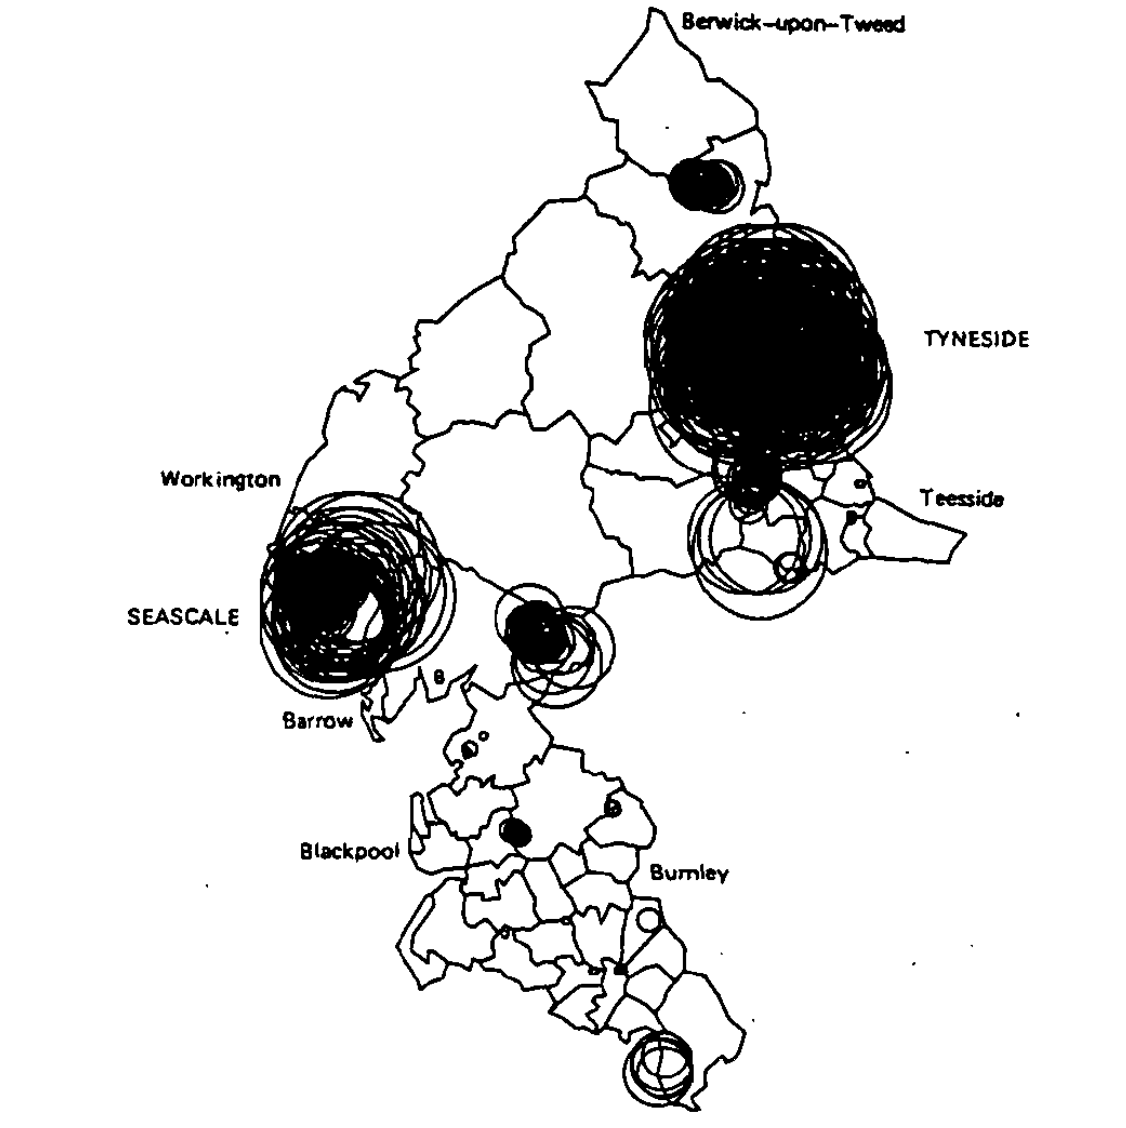
\includegraphics[width=0.6\textwidth]{figures/openshaw.png}
	
	\footnotesize
\textit{Geographic analysis machine \cite{openshaw1987mark}}
	
	\medskip
	\hrule
	\medskip
	
	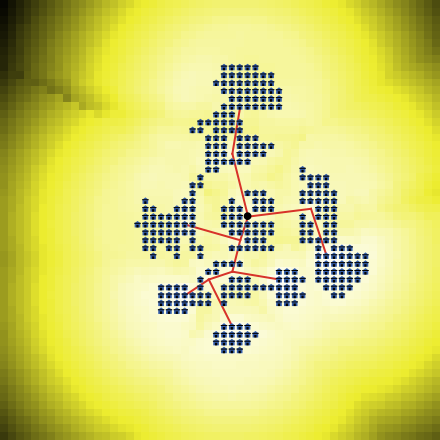
\includegraphics[width=0.55\textwidth,height=0.3\textheight]{figures/intro_RBD_lattice.png}
	
	\footnotesize
\textit{Hybrid urban morphogenesis \cite{raimbault2014hybrid}}
	

	\end{column}
	\vrule{}
	\begin{column}{0.5\textwidth}
	\centering
	
	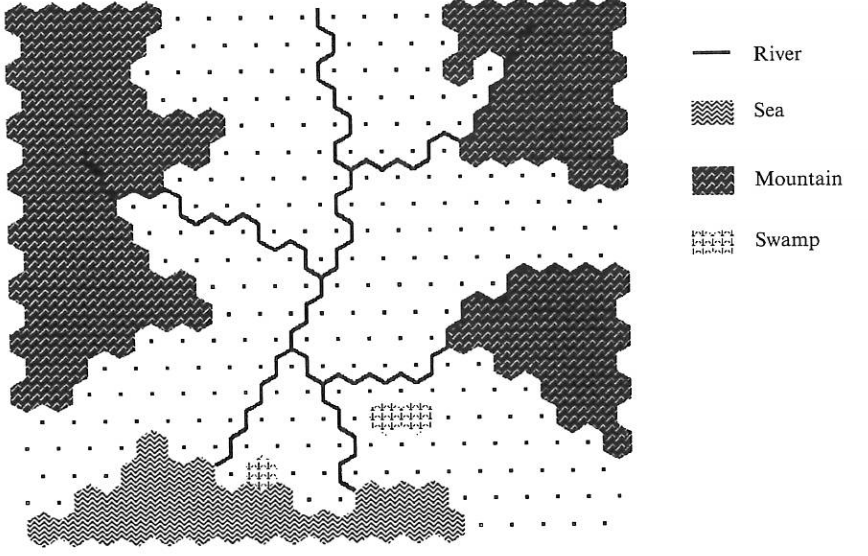
\includegraphics[width=0.7\textwidth]{figures/simpop1.png}
	
	\footnotesize
\textit{Simpop 1 model \cite{sanders1997simpop}}

	\medskip

	\hrule
	
	\medskip

	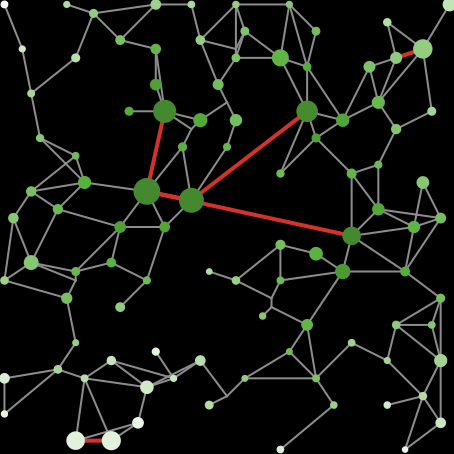
\includegraphics[width=0.6\textwidth]{figures/setup_synth_1_tick100.png}
	
	\footnotesize
	\textit{SimpopNet model \cite{schmitt2014modelisation}}
	
	\end{column}


\end{columns}

}


\sframe{Current trends and challenges in (geo-)simulation}{

% 
%\centering
%\justify

% We first survey the current trends and explicit the positioning of OpenMOLE's philosophy within these.

\textbf{Key domains: } quantifying urban growth and form, mining spatio-temporal data, geosimulation, multi-scalar approaches \cite{behnisch2018trends}.

\medskip

\textbf{Challenges: }

\begin{itemize}
	\item \cite{perez2016agent} key challenges in ABM for planning: addressing complexity in a clean way, addressing multi-dimensionality, feasible trajectories, participatory planning.
	\item Simulation models \cite{banos2013pour}: interdiscplinarity, data-driven models, exploration of models, multi-objective issues, reproducibility and reuse of models, coupling models.
\end{itemize}


\medskip

\textbf{Future ?} \cite{banos2017knowledge} deeper and integrated knowledge; \cite{arribas2018geography} new geographic data science?


}

\sframe{OpenMole's positioning}{

\textit{A qualitative shift in knowledge that can be extracted from a simulation model with model exploration methods.}

\medskip

Success stories: SimpopLocal \cite{schmitt2014half}, Marius \cite{10.1371/journal.pone.0138212}, Ecological modeling \cite{lavallee2018dynamical}, epidemiology \cite{arduin2018modelisation}, etc.

\medskip

\textbf{Key features: }

\begin{itemize}
	\item Unique role of complementary axis of computation environment access, methods providing, and model embedding.
	\item Iterative and integrated construction of models and theories, using all dimensions of knowledge enhanced by simulation and computation (modeling, theory, empirical, data, methods, tools \cite{raimbault2017applied}.
	\item Coupling models and reproducibility at the core of the workflow approach \cite{passerat2017reproducible}
\end{itemize}


}


\sframe{Citation network analysis (full)}{

% % A citation network mapping helps situating it in the broader context of computational science.

\centering

%\vspace{-1.5cm}
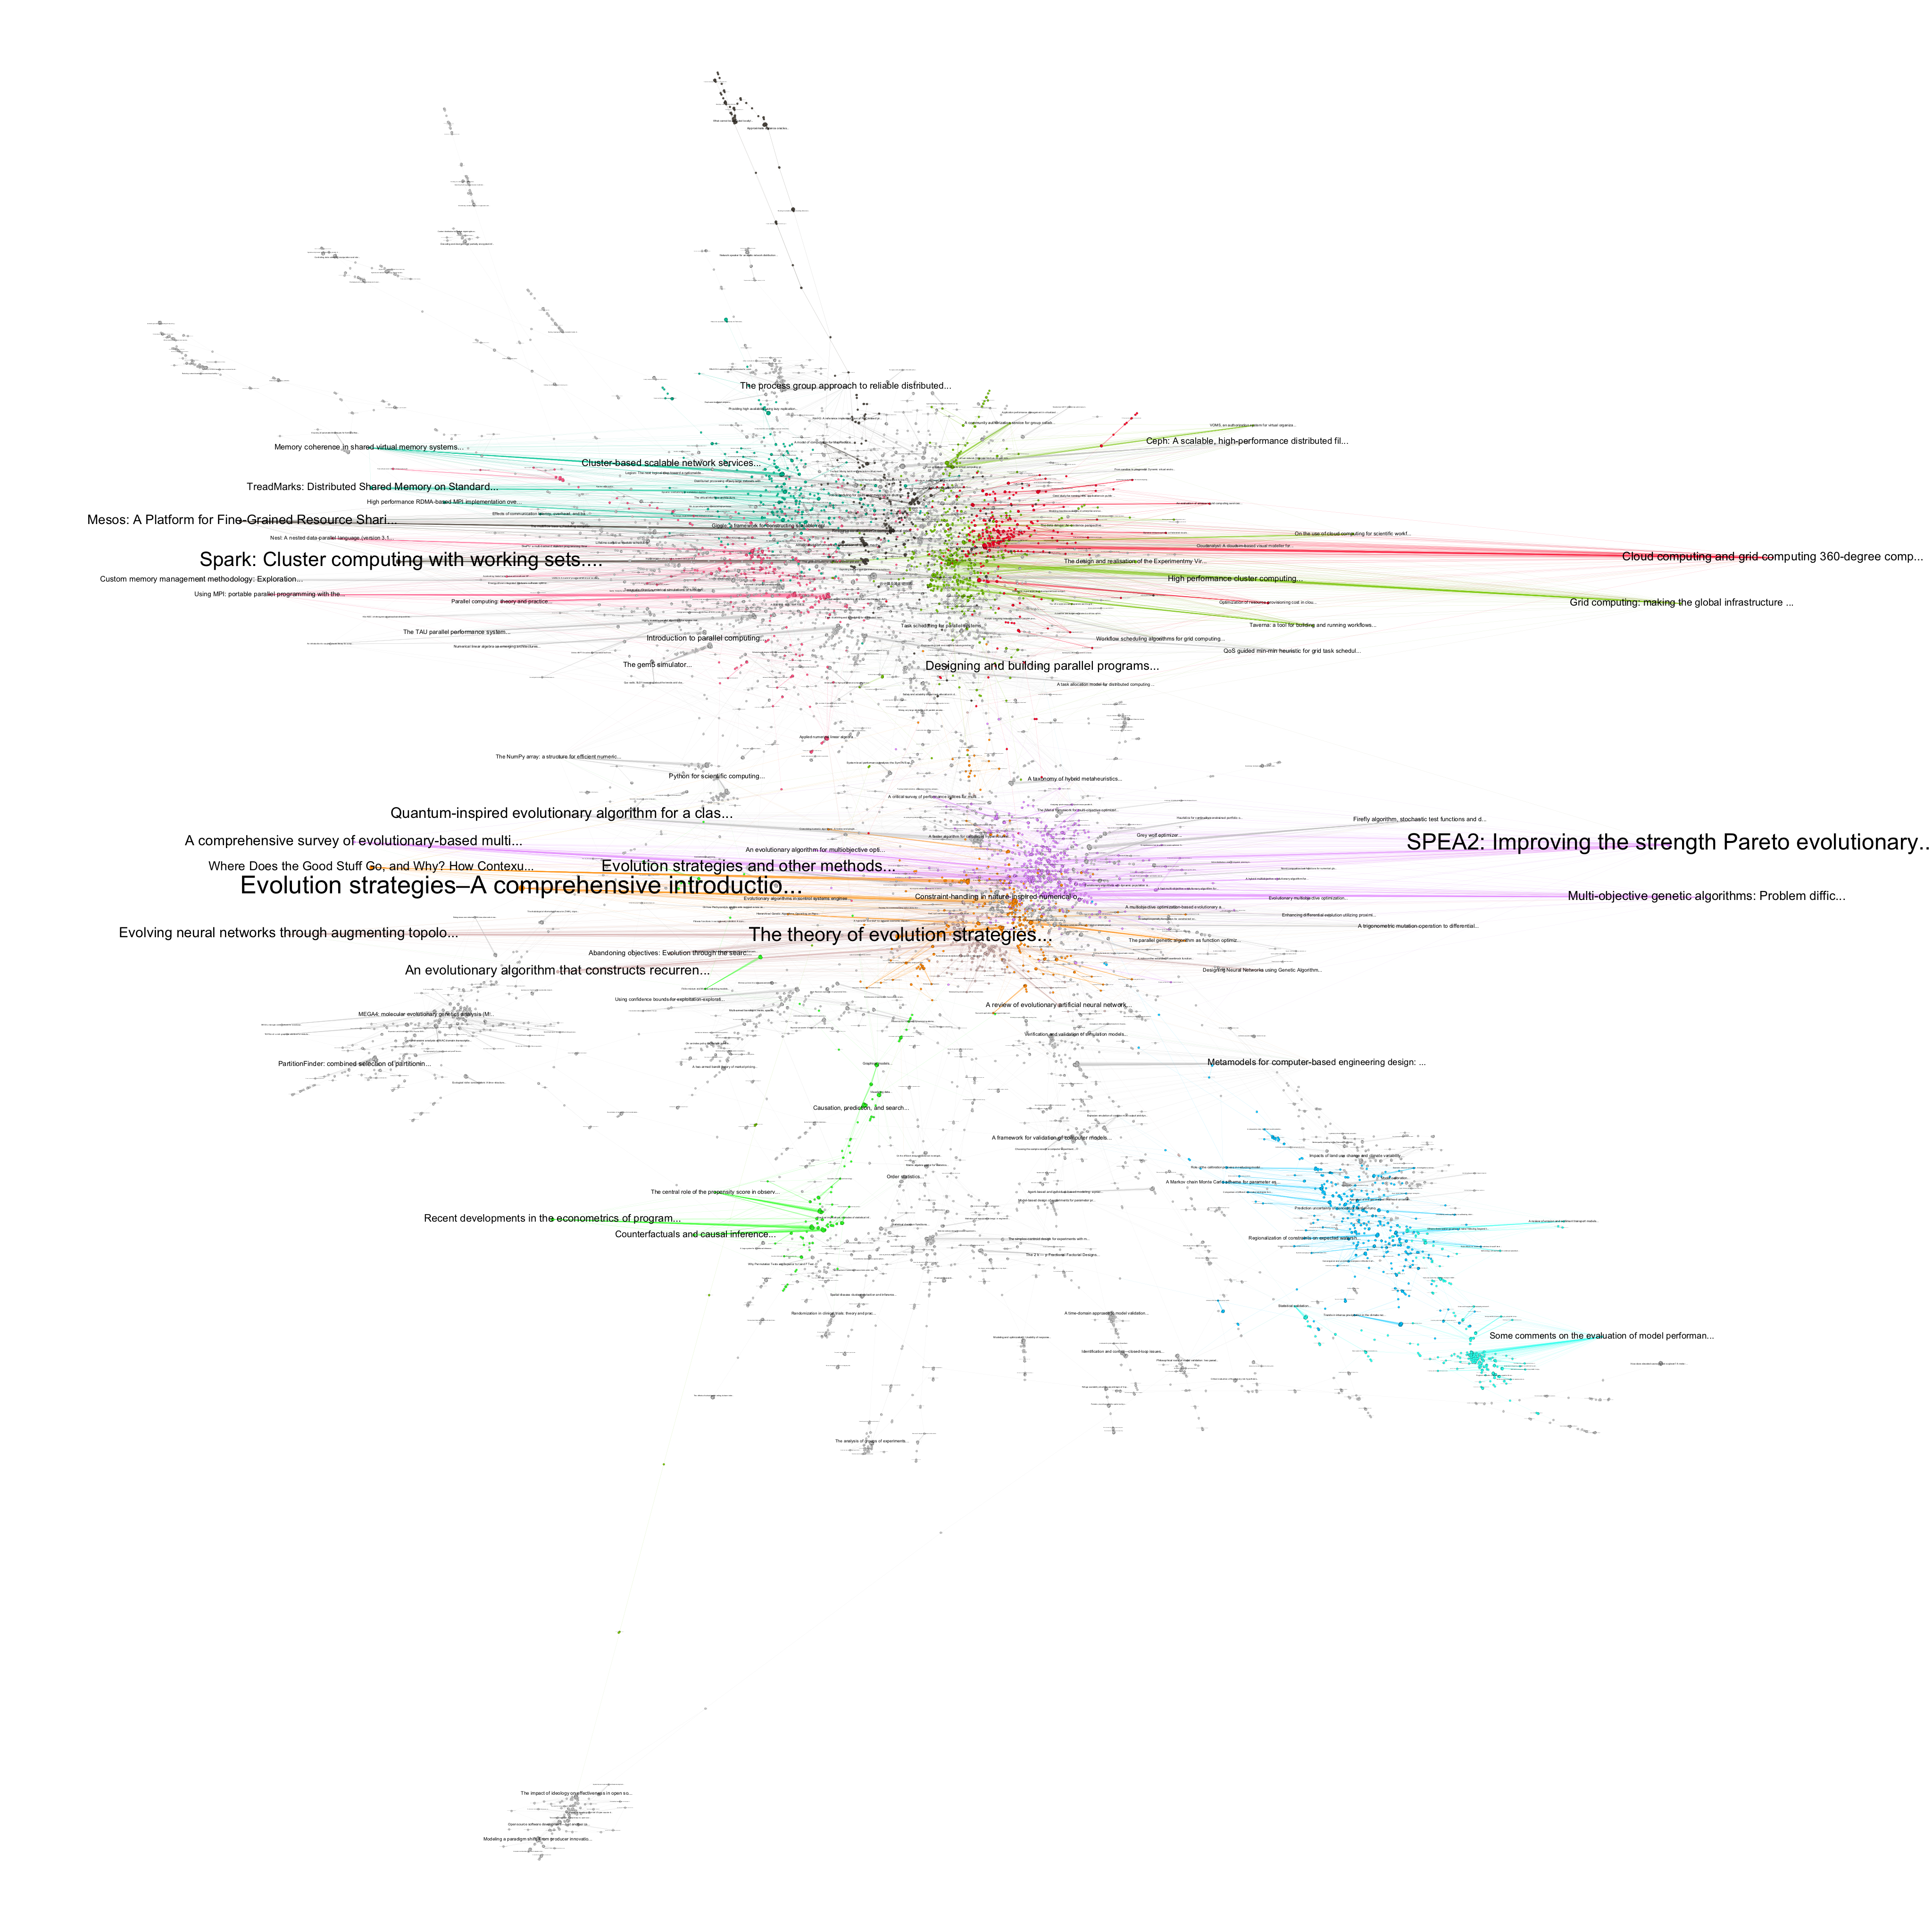
\includegraphics[width=1.2\textwidth,trim={1cm 0 1cm 1cm}]{figures/citnw_sampled.png}

}


\sframe{Citation network analysis (OpenMOLE)}{

\centering

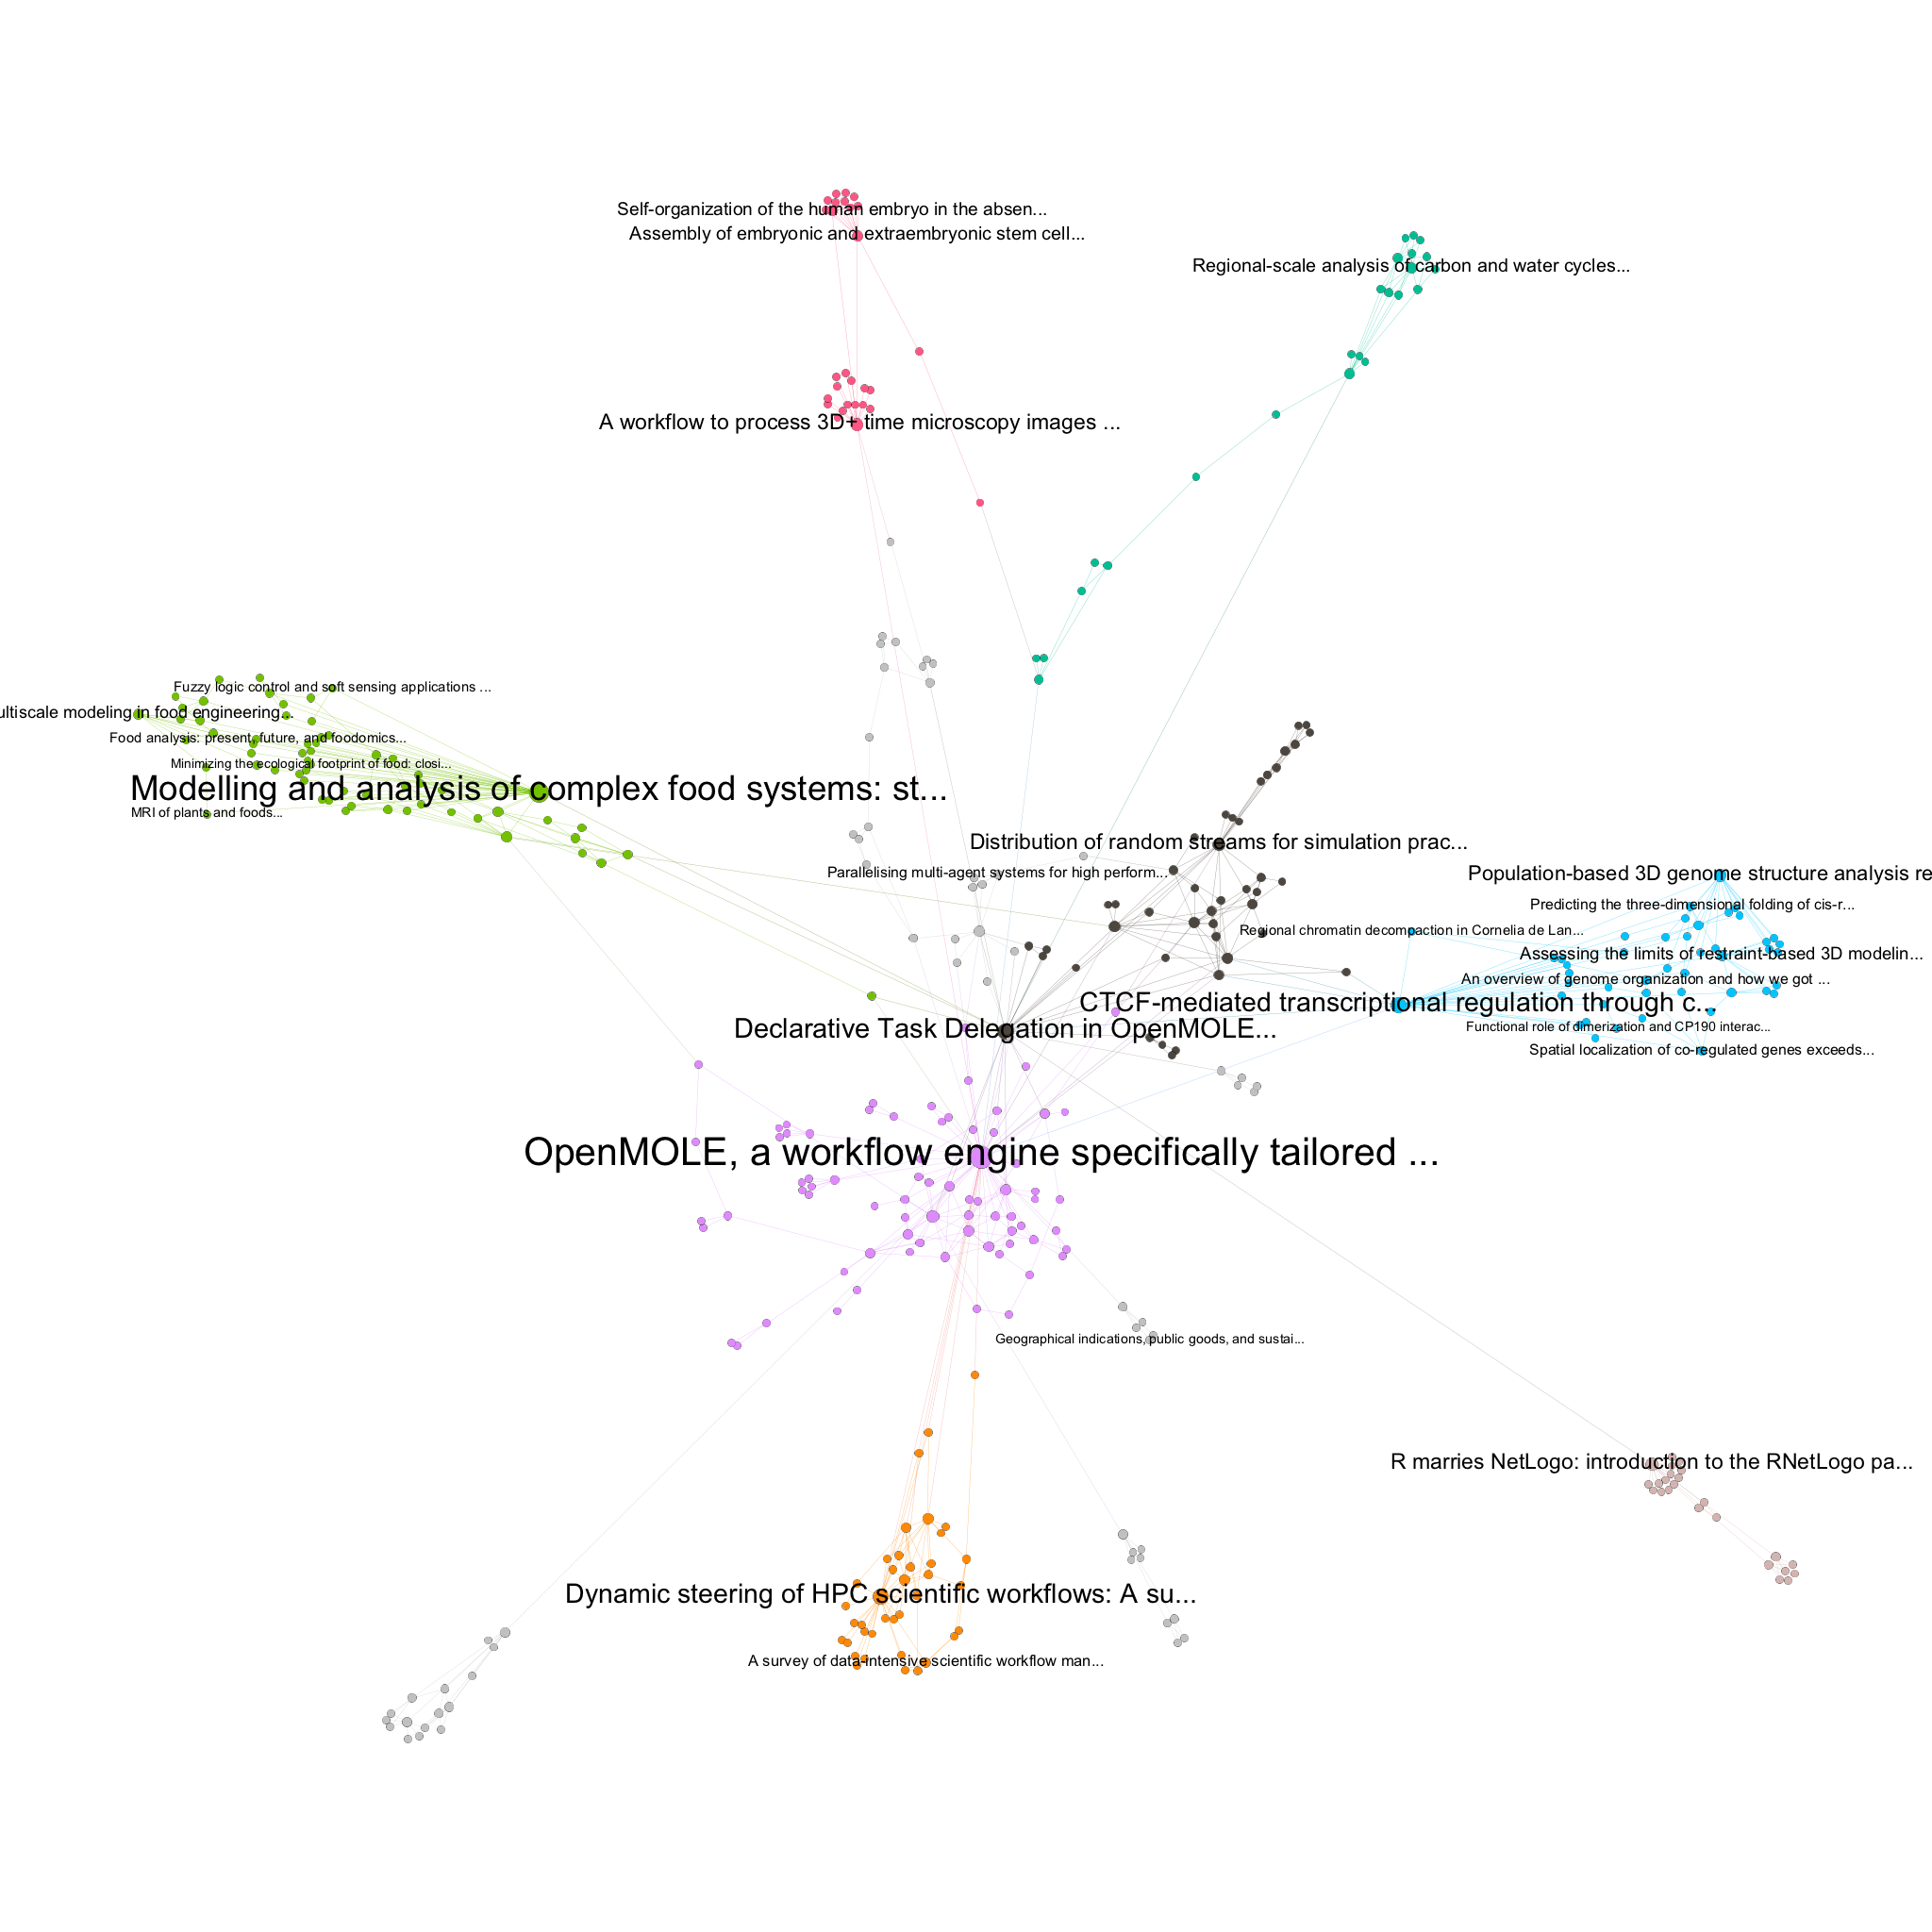
\includegraphics[width=\textwidth]{figures/oml_depth3_core.png}
}




\sframe{Perspectives and open issues for simulation in geography}{

%We then propose a grasp on some future perspectives, by detailing examples of crucial research questions on simulation models in geography that remain open, including in particular, first generic issues such as

% plan (generic + specific to spatio-temporal modeling)

\textit{Some of crucial issues :}

\medskip

\textbf{Generic issues: }
\begin{itemize}
	\item Overfitting in simulation models
	\item Model coupling
	\item Direct and inverse mapping
	\item Stochasticity
\end{itemize}

\medskip

\textbf{Specific issues to spatio-temporal systems: }
\begin{itemize}
	\item Spatio-temporal non-stationarity
	\item Spatio-temporal synthetic data
\end{itemize}




}





\sframe{Dealing with overfitting}{

% (i) the development of multi-modeling techniques that explicitly account for overfitting for simulation models;

\textit{When do additional parameters actually capture new dimensions of the simulated system ? i.e. when does fit improvement is not only due to more degree of freedom ?}

\medskip

$\rightarrow$ Crucial for parcimonious models, which can be used then as building bricks for more complex models.

\medskip

\begin{itemize}
	\item Black-box brutal data explanation ?
	\item Extension of AIC-type measures ?
	\item Multi-objective optimisation with degrees of freedom ?
\end{itemize}


}


\sframe{Model coupling}{

% (ii) a better understanding of model coupling
% (includes multi-scale more or less)
% -> robust definition / classification of models etc

\textit{Definition/theory/quantification of model coupling ?}

\medskip

$\rightarrow$ Crucial for interdisciplinarity, reproducibility and the reuse of models; crucial for multi-scalar approaches (downward causation); crucial for model benchmarking.

\medskip

\begin{itemize}
	\item Model-independent notion of ``coupling-strength'' ?
	\item Covariance structures ?
	\item Causal graphs ?
\end{itemize}

}


\sframe{Direct and inverse mapping}{

% (iii) the development of adaptative direct and inverse mapping methods;
% inverse problems / feasible space

\textit{How to have a comprehensive overview of strongly non-linear simulation models mapping ?}

\medskip

$\rightarrow$ Feasible space and unexpected patterns (PSE algorithm \cite{10.1371/journal.pone.0138212}); dealing with equifinality.

\medskip

\begin{itemize}
	\item Inverse problem heuristics being currently tested in OpenMOLE
	\item Iterative approach to determine main patterns in the mapping ?
\end{itemize}

}


\sframe{Handling stochasticity}{

% (iv) a better handling of stochasticity in ``real-world'' models;

\textit{How to handle stochastic models during genetic algorithm calibration or exploration ?}

\medskip

$\rightarrow$ Crucial for more data-driven and ``real-world'' models; crucial for a robust knowledge extracted from simulation models.

\medskip

\begin{itemize}
	\item Deal with ``real-world'' noise patterns
	\item An embedding approach tested in OpenMOLE to deal with noisy fitness
	\item A bayesian approach to calibration (ABC) also currently tested
\end{itemize}



}

\sframe{Spatio-temporal modeling issues: non-stationarity}{

%  and secondly issues which are more specific to spatio-temporal models, such as (v) the understanding of spatio-temporal non-stationarity, possibly through the intermediate of limit links between agent-based approaches and system dynamics approaches;

\textit{How to understand and include spatio-temporal non stationarity in empirical analysis / in model simulations and calibration ?}

\medskip

$\rightarrow$ Intrinsic complexity of spatial systems; crucial for multi-scalar approaches.

\medskip

\begin{itemize}
	\item Link between non-stationarity and non-ergodicity
	\item Link between ABM approaches and dynamical systems approaches, towards hybrid approaches \cite{banos2015importance}
\end{itemize}


}


\sframe{Spatio-temporal synthetic data}{

% and (vi) methods to generate synthetic spatio-temporal data to be used for broader sensitivity analyses.

\textit{How to extend sensitivity analyses to spatial initial conditions ? How to generate spatial synthetic data ?}

\medskip

$\rightarrow$ Crucial for the robustness of spatial simulations

\medskip

\begin{itemize}
	\item First work in the case of density grids in territorial systems \cite{cottineau2017initial}
	\item Extend to other disciplines: ecology, geosciences
	\item Towards a generic library integrated in OpenMOLE
\end{itemize}

}





\sframe{An integrated view}{
	
	% graph between different open issues
	
	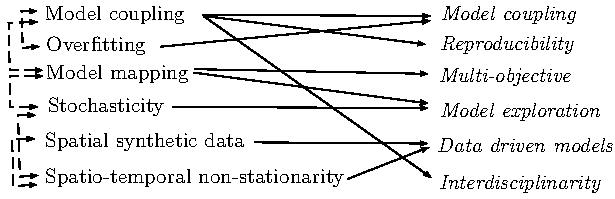
\includegraphics[width=\textwidth]{figures/directions.pdf}
	
}


\sframe{Applied perspectivism to couple modeling approaches}{

% We finally describe an epistemological framework integrating several of these issues, which applies Giere's perspectivism to the effective coupling of simulation models, and that we call ``applied perspectivism''. This framework should foster the development of integrative theories through the coupling of perspectives, and therefore of models.

% link it with knowledge framework

Giere's perspectivism \cite{giere2010scientific}: a ``third way'' beyond constructivism-realism: \textit{Any scientific knowledge construction process as a perspective by an agent to answer a purpose with a media (model)}.

\medskip

Applied knowledge framework proposed by \cite{raimbault2017applied} to study [complex] systems: \textit{co-evolution} of cognitive agents and knowledge domains, through the intermediate of perspectives.

\medskip

\textbf{Applied perspectivism principles:}
\begin{itemize}
	\item Foster consistence of perspectives and their communication (Banos' virtuous spiral between disciplinarity and interdisciplinarity)
	\item Importance of reflexivity to ease the coupling of perspectives
	\item New model exploration methods increase the integration between knowledge domains
	\item Coupling of models as a possible medium to couple perspectives (transfer hypothesis)
\end{itemize}

\medskip

\textit{Still to be formalized, specified as possible implementations, and experimented.}


}






\sframe{Conclusion}{


\justify

%\vspace{-1cm}

%$\rightarrow$ 

\textit{Significant accomplishments beyond disciplines, construction of new research practices (see the satellite presentations)} $\rightarrow$ still much to do ? (e.g. how to put into practice ? how to achieve true integration ? etc.)

\bigskip

\textbf{\textit{``La route est longue mais la voie est libre''}}

\bigskip

\textbf{\textit{You need OpenMOLE and OpenMOLE needs you !}} (win-win interdisciplinary relations): apply to the summer school !\\
\texttt{https://exmodelo.org/}

\bigskip
\bigskip
\bigskip

\footnotesize

\textbf{Related works on epistemological considerations}

Raimbault, J. (2017, December). An Applied Knowledge Framework to Study Complex Systems. In Complex Systems Design \& Management (pp. 31-45). arXiv:1706.09244.

\smallskip


Raimbault, J. (2018). Caract{\'e}risation et mod{\'e}lisation de la co-{\'e}volution des r{\'e}seaux de transport et des territoires (Doctoral dissertation, Université Paris 7 Denis Diderot). \url{https://halshs.archives-ouvertes.fr/tel-01857741}




%\smallskip

%\textbf{Open repository} at \texttt{https://github.com/JusteRaimbault/UrbanGrowth}\\\smallskip
%\textbf{Acknowledgments}: thanks to the \textit{EGI} for access to the infrastructure.


}






\sframe{Reserve slides}{

\centering

\Large

\textbf{Reserve Slides}

}



%%%%%%%%%%%%%%%%%%%%%
\begin{frame}[allowframebreaks]
\frametitle{References}
\bibliographystyle{apalike}
\bibliography{/Users/juste/ComplexSystems/CityNetwork/Biblio/Bibtex/CityNetwork,biblio}
\end{frame}
%%%%%%%%%%%%%%%%%%%%%%%%%%%%




\end{document}









